\documentclass[a4paper,11pt,exos]{nsi} % COMPILE WITH DRAFT
\usepackage{pifont}
\usepackage{hyperref}
\usepackage{fontawesome5}

\pagestyle{empty}

\begin{document}
\classe{\seconde}
\titre{Battle d'argumentation mathématique}
\maketitle

\exo{ \faClock\hspace*{.1cm} 1 min}
Que fait le programme Python suivant ?\\
\begin{pyc}
    \begin{minted}{python}
        from random import randint
        d=randint(1,6)
        print(d)
    \end{minted}
\end{pyc}


\exo{ \faClock\hspace*{.1cm} 1 min}
Que fait le programme Python suivant ?\\
\begin{pyc}
    \begin{minted}{python}
    d1 = 4
    d2 = 2
    d = max(d1,d2)
    print(d)
    \end{minted}
\end{pyc}

\exo{ \faClock\hspace*{.1cm} 1 min}
Que fait le programme Python suivant ?\\
\begin{pyc}
    \begin{minted}{python}
    compteur = 0
    for i in range(10):
        d = randint(1,6)
        if d == 6:
            compteur = compteur + 1
    print(compteur)
    \end{minted}
\end{pyc}

\newpage

\exo{ \faClock\hspace*{.1cm} 2 min}
On reprend le programme de l'exercice 3 :

\begin{pyc}
    \begin{minted}{python}
    compteur = 0
    for i in range(10):
        d = randint(1,6)
        if d == 6:
            compteur = compteur + 1
    print(compteur)
    \end{minted}
\end{pyc}
Quelle est la probabilité que le programme suivant affiche \mintinline{python}{0}  ?\\


\exo{ \faClock\hspace*{.1cm} 1 min}
Dans le jeu « Traversée de la rivière », la stratégie des saut moyens consiste à lancer deux dés et à avancer du nombre de cases égal au maximum des deux dés.\\[.5em]
Comment peut-on simuler un saut moyen à l'aide d'un programme Python ?

\exo{ \faClock\hspace*{.1cm} 2 min}
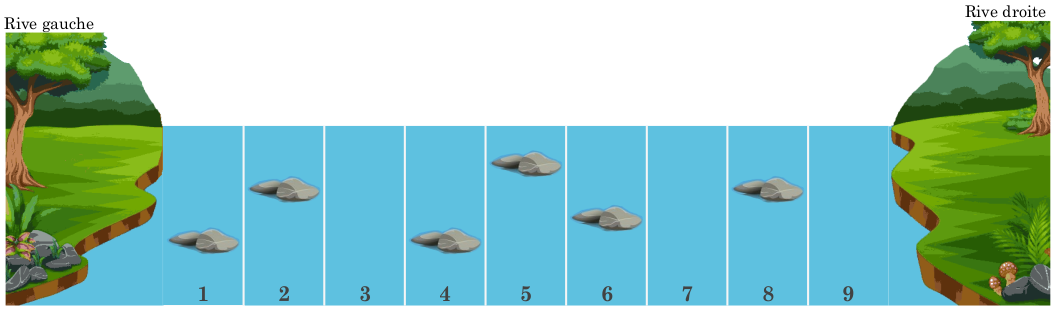
\includegraphics[width=17cm]{image.png}\\
Quelle est la probabilité de tomber à l'eau au premier saut avec la stratégie des sauts moyens ?

\newpage
\exo{ \faClock\hspace*{.1cm} 2 min}
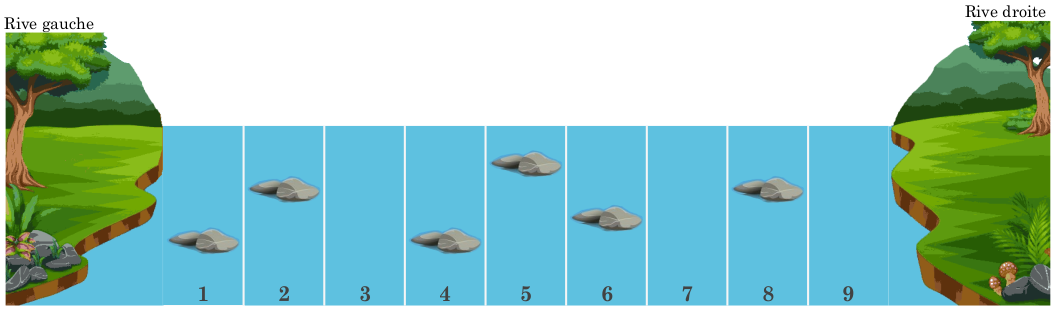
\includegraphics[width=17cm]{image.png}\\
Comment simuler une partie de « Traversée de la rivière » avec la stratégie des sauts moyens ?\\[.5em]
Donner l'idée de l'algoritme sans l'écrire en Python.

\exo{ \faClock\hspace*{.1cm} 2 min}
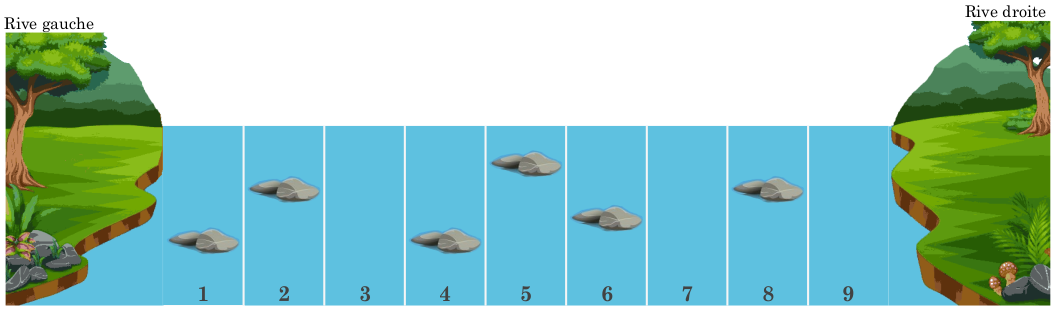
\includegraphics[width=17cm]{image.png}\\
Comment simuler 100 parties de « Traversée de la rivière » avec la stratégie des sauts moyens et afficher le nombre de réussites ?\\[.5em]
Donner l'idée de l'algoritme sans l'écrire en Python.

\end{document}